\section{Proposed approach}



\label{chap:PURE}

%\subsection{Introduction}


%In this article, we describe a novel tool for Predicting Upstream REgulators (PURE) that can perform a causal analysis and infer the cause of a set of measured gene expression changes. 
In this chapter, we describe a novel causal analysis tool for predicting upstream regulators that can infer the cause of a set of measured gene expression changes. 
Given a set of differentially expressed genes between samples with studied phenotype and control samples, we would analyzes more  than 5,000 CDTs and their 330,659 known associations with human genome, 187,759 associations with mouse genome, and 161,323 associations with the rat genome as described in the Comparative Toxicogenomics Database~\cite{mattingly2006comparative}. 
 
% \hfill
 
In the following subsections, we present the hypotheses tested in the study and the approach to calculate the significance score for each hypothesis.
%We propose  assessment criteria of the performance of PURE and compare it with four classical methods, namely Over Representation Analysis using hypergeometric test~\cite{DraghiciOE2:2003}, Kolmogorov-Smirnov (KS)\cite{massey1951kolmogorov}, Wilcoxon\cite{wilcoxon1945individual}, FGSEA~\cite{korotkevich2021fast}, and a commercial tool, namely Ingenuity Pathway Analysis~\cite{kramer2013causal}. 
%The result shows that our method outperforms existing methods in term of both the ability of identifying the causal CDT, as well as in terms of the number of false positives yielded by each method.

%\subsection{Methods}

\subsection{Knowledge base}
First, we would preprocess the network of drug-gene interactions from the Comparative Toxicogenomics Database~\cite{mattingly2006comparative} that provides manually curated information about associations between more than 5,000 CDTs and tens of thousands of genes from many species including human, mouse, rat, etc. These data include the chemical family, the CDT-gene, and CDT-disease relationships.
There are various types of relationships between a CDT and targeted or affected genes, such as increase/decrease expression, increase/decrease abundance, or increase/decrease methylation.
In this analysis, since our goal is to analyze gene expression measurements, we would focus on  those effects leading to an expression increase or decrease. Henceforth, these will be referred to as ``activation'' and ``inhibition'' effects.



\subsection{Two hypotheses}

For each CDT in the database, we would consider two hypotheses:

\begin{itemize}
\item Hypothesis 1 (H1): the level of the CDT is higher in the phenotype compared to the control.%; and hence, enhances expressions of the downstream genes via the direct interaction edges.
\item Hypothesis 2 (H2): the level of the CDT  is lower  in the phenotype compared to the control (or completely absent).%; and hence, the downstream genes are not regulated properly.
\end{itemize}

\subsection{Statistical significance}


Let $G_{DE}$ be the set of differentially expressed genes available in the gene expression profile; $C_{KB}$ be the set of all CDTs in the knowledge base (KB); $G_{KB}$ be the set of genes in the KB, and $E_{KB}$ be the set of edges that represents the associations between CDTs and genes in the KB. 
%where $A \in C_{CTD}$ is a chemical, $x \in G_{CTD}$ reflects a gene, and an edge $e_{A,x} \in E_{CTD}$ represents a relationship between the drug $A$ and gene $x$.

\begin{figure*}
\centering
  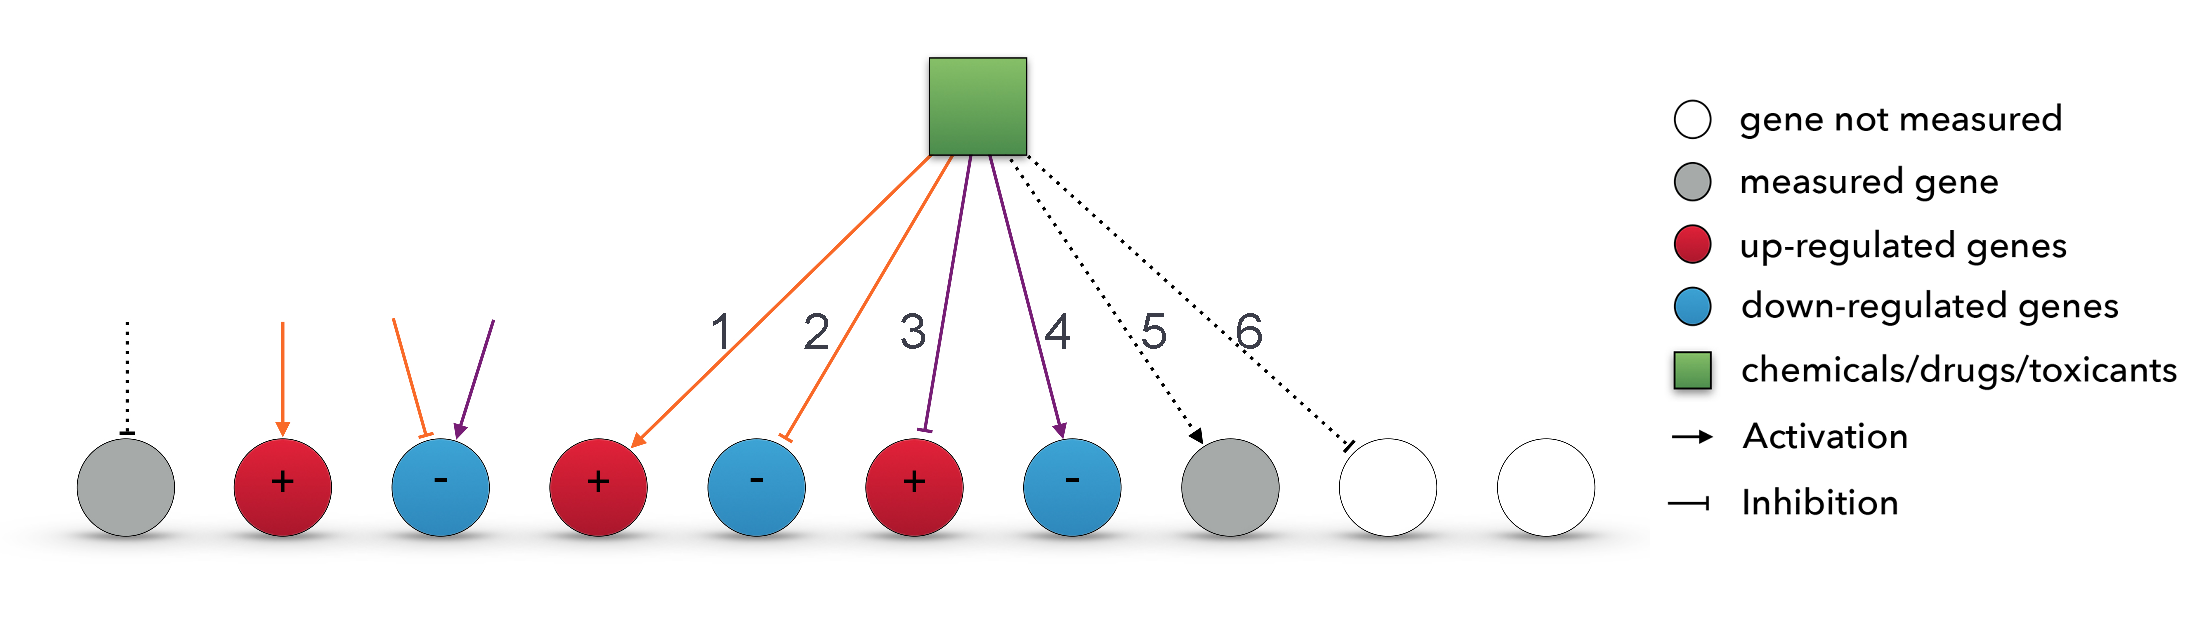
\includegraphics[width=0.9\linewidth]{Figures/SecondEvidence.pdf}
  \caption{Illustration of different types of genes available in the Comparative Toxicogenomics Database and gene expression profile, and their relationships with the chemical. The significance of a chemical/drug/toxicant (green box) in each hypothesis is assessed using a statistical test based on the number of up- or down-regulated DE genes and their associations with the drug. The orange edges (e.g. 1 and 2) are the ones that support the hypothesis that level of studied chemical/drug/toxicant is higher in the phenotype compared to the control while the purple ones (e.g. 3 and 4) are supporting the hypothesis that its level is lower compared to the control.}
  \label{fig:SignificantDrug}
\end{figure*}

We define G as  the set of genes included in both $G_{DE}$ and $G_{KB}$, i.e.  $G_{DE} \cap G_{KB}$. Subsequently, $C \subseteq C_{KB}$  and $E \subseteq E_{KB}$ represent the set of all CDTs and their corresponding associations with those genes in $G$ available in the knowledge base. These sets are formally defined as follows:

\begin{equation}C = \{c \in C_{KB} \mid \exists g \in G \land \exists e_{c,g} \in E_{KB} \}\end{equation}

and 

\begin{equation} E = \{ e_{c,g} \mid \exists c \in C \land  \exists g \in G \ \land  e_{c,g} \in E_{KB} \} \end{equation}

%Let $G^{+}\subseteq G$ and $G^{-}\subseteq G$ be the list of up- and down-regulated DE genes, respectively. 

where $e_{c,g}$ denotes an edge from an upstream CDTs $c$ to targeted gene $g$ representing their relationship described in the Comparative Toxicogenomics Database. The sign of the edge, $s(e_{c,g})$, reflects the type of the association, namely positive ($+$) for an activation and negative ($-$) for an inhibition edge. Also, we denote $s(g)$ the sign of the DE gene $g$ which is positive if $g$ is up-regulated, and negative, otherwise. 

Each edge $e \in E$ is labeled whether it is supporting either of the testing hypotheses (Fig.~\ref{fig:SignificantDrug}). 
For example, if an edge is activation and its targeted DE gene is indeed up-regulated, the edge supports the hypothesis 1. 
%Similarly, an inhibition edge connected with a down-regulated DE gene is also backing this hypothesis. 
In essence, an edge is considered to be supporting the hypothesis 1 when its sign, $s(e_{c,x})$, is aligned with the sign of its targeted DE gene, namely $s(e_{c,g}) = s(g)$. 
Such edges are colored orange in Fig.~\ref{fig:SignificantDrug}. 
Edges whose signs are opposite with the expression direction of their targeted DE genes are considered as a supporting evidence for the hypothesis 2, and are colored purple in  Fig.~\ref{fig:SignificantDrug}. 
Notice that $E^{H1}$ and $E^{H2}$ are the two mutually exclusive sets of edges that support the first and second hypothesis, respectively, because an edge $e \in E$ must support either the hypothesis 1 or hypothesis 2, but not both. Formally, $E^{H1} \cap E^{H2} = \emptyset$ and  $E^{H1} \cup E^{H2} = E$. 

For each chemical $c \in C$, a statistical score, i.e. p value, for each aforementioned hypothesis is then computed using the one-sided Fisher's exact test. Without losing generality, let us discuss the hypothesis 1. First, a confusion matrix is constructed as in Table \ref{ConfusionMatrix}, where $l$, $k$, $m$, and $n$ are the number of edges related to $c$ that support the hypothesis, the number of edges related to $c$ that do not support the hypothesis, the number of edges not related to $c$ that support the hypothesis, and the number of edges not related to $c$ that do not support the hypothesis, respectively. 
The probability of this observed contingency under the null hypothesis is defined as follows:
\begin{equation}
p = \frac{ {l+k \choose l}{m+n \choose m}}{{\|E\| \choose l + m}}
\end{equation}
where $\|E\| = (l+k+m+n)$ is the number all edges in $E$. 

The p value of the one-sided Fisher's exact test is the sum of the probabilities of all contingency tables that have the number of edges supporting the H1 more than $l$ where the number of edges related to the compound C and the number of edges supporting the H1 are unchanged.

Notice that because an edge supporting H1 is against H2 and vice versa, the contingency matrix for H2 can be obtained by swapping the columns of the observed contingency matrix of H1. Hence, the p value for the H2 can also be derived from these four numbers.


Finally, we use the false discovery rate (FDR) to correct the p values for multiple comparisons~\cite{Benjamini:1997}.

\begin{table}
\caption{For each chemical/drug/toxicant $c$, a contingency table is constructed. Here, \emph{l}, \emph{k}, \emph{m}, and \emph{n} are the number of edges coming from $c$ that support the hypothesis 1 (H1), the number of edges coming from $c$ that do not support the H1, the number of edges not coming from $c$ that support the H1, and the number of edges not coming from $c$ that do not support the H1, respectively. Note that the edges that support H1 are against the hypothesis 2 (H2), and vice versa. Hence, a similar contingency table for H2 can be constructed using these four numbers.}
\begin{center}
\begin{tabular}{c|cc}
&  Supporting H1& Against H1\\
\hline
Related to $c$& \emph{l} & \emph{k} \\
 Not related to $c$&\emph{m}& \emph{n}  \\
%\hline 
%Total & $\|E1\|$ & $\|E2\|$ & $\|E\|$
\end{tabular}
\end{center}
\label{ConfusionMatrix}
\end{table}%






%\subsection{Conclusion}
%
%The most important contribution of PURE is that it can infer the CDT responsible for the gene expression changes, which in turn causes the observed phenotype. This crucial ability is expected to be useful for the correct identification of the presence of chemicals, drugs or toxicants in new and unknown phenotypes.  Moreover, PURE can identify the CDT that can revert disease-induced gene expression changes. This capability is expected to be useful in any drug repurposing application. In fact, this approach coupled with a pathway analysis, was able to repurpose methylprednisolone to treat severe symptoms related to hyper-inflammation of COVID-19 patients, very early in the pandemic, at a time when the WHO's recommendation was against the use of steroids~\cite{DraghiciCOVID:2021}.
% 
%The proposed approach was validated using 16 gene expression data sets from 3 different species where the true CDTs that caused the phenotypes were known. PURE correctly identified the CDT used in 11 out of 16 data sets (7 of which the true CDTs were ranked at the top). We also compared PURE to 5 other methods including a commercial tool, IPA. PURE outperformed all other methods in terms of the rank of the true CDT and the number of false positives in the list of significant CDTs.